\documentclass[12pt, letterpaper, twoside]{article}
\usepackage[utf8]{inputenc}
\usepackage{graphicx}
\graphicspath{ {images/} }
 
\title{Dogs}
\author{Martyna Iwaniec I MA PJN}
\date{April 2020 }
 
\begin{document}

\maketitle
\begin{abstract}
This \LaTeX{} document is about dogs. Because everyone likes dogs.
\end{abstract}

\tableofcontents
 
\section{Introduction}
This is the introduction. Dogs (Canis lupus familiaris) are domesticated mammals, not natural wild animals. They were originally bred from wolves. They have been bred by humans for a long time, and were the first animals ever to be domesticated. There are different studies that suggest that this happened between 15.000 and 100.000 years before our time. The dingo is also a dog, but many dingos have become wild animals again and live independently of humans in the range where they occur (parts of Australia).

% This line here is a comment. You don't have to worry about it.
 
Some of the \textbf{cutest}
dogs are \underline{puppies} 
and \textbf{\textit{strays}}.

Here is a picture of a cute puppy:
\begin{center}
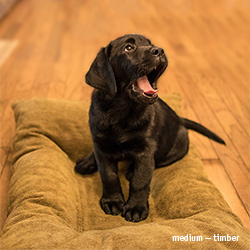
\includegraphics{puppy}
 
His name is Reksio.
\end{center}

Dogs are called \emph{man's best friend} 
because they fit into human lives.

\textit{Dogs have lived with humans \emph{for a very long time} 
and
they will for as long as humans exist.}

\textbf{Some of the greatest \emph{friendships} 
in the history 
were between humans and their dogs.}


\section{First Chapter}
 
 \begin{figure}[h]
    \centering
    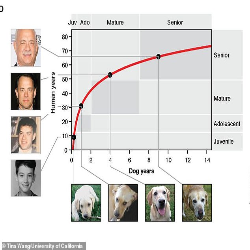
\includegraphics[width=0.25\textwidth]{dog_years}
    \caption{Dog years and human years}
    \label{fig:dog_years}
\end{figure}
 
As you can see in the figure \ref{fig:dog_years}, dogs grow old differently than humans.

\begin{itemize}
  \item Dogs are regarded as members of a family by their owners.
  \item Having a dog is like having a baby, but easier.
  \item Having a dog is good for your mental and physical health.
\end{itemize}

\begin{enumerate}
  \item Dogs are very loyal.
  \item Dogs are great playmates.
  \item Dogs are a big responsibility.
\end{enumerate}

\section{Second Chapter}

Dogs are not very good at math.
\[ Dog=love ^2 \]
But if they were, they would learn things like 
\begin{equation}
E=mc^2
\end{equation}

They would also study mathematical operators like $\sin(\beta)$, $\cos(\alpha)$, $\log(x)$ etc.

Here are some random tables:

\begin{center}
\begin{tabular}{ c c c }
1 & 2 & 3 \\ 
1 & 2 & 3 \\  
1 & 2 & 3    
\end{tabular}
\end{center}
 
\begin{center}
\begin{tabular}{ |c|c|c| } 
\hline
1 & 2 & 3 \\ 
1 & 2 & 3 \\  
1 & 2 & 3 \\  
 \hline
\end{tabular}
\end{center}

\begin{center}
    The end
\end{center} 

\end{document}
